\begin{pages}
    \begin{Rightside}
    \selectlanguage{greek}
        \beginnumbering
        \pstart[
        			\chapter{Ὁ ἕβδομος ἄγγελος σαλπίζει}
        			\markboth{The Seventh Angel Sounds}
				]
		Καὶ ἐδόθη μοι κάλαμος ὅμοιος ῥάβδῳ, λέγων Ἔγειρε καὶ μέτρησον τὸν ναὸν τοῦ Θεοῦ καὶ τὸ θυσιαστήριον καὶ τοὺς προσκυνοῦντας ἐν αὐτῷ. καὶ τὴν αὐλὴν τὴν ἔξωθεν τοῦ ναοῦ ἔκβαλε ἔξωθεν καὶ μὴ αὐτὴν μετρήσῃς, ὅτι ἐδόθη τοῖς ἔθνεσιν, καὶ τὴν πόλιν τὴν ἁγίαν πατήσουσιν μῆνας τεσσεράκοντα δύο.
		\pend
		\pstart
		καὶ δώσω τοῖς δυσὶν μάρτυσίν μου, καὶ προφητεύσουσιν ἡμέρας χιλίας διακοσίας ἑξήκοντα περιβεβλημένοι σάκκους. Οὗτοί εἰσιν αἱ δύο ἐλαῖαι καὶ αἱ δύο λυχνίαι αἱ ἐνώπιον τοῦ Κυρίου τῆς γῆς ἑστῶτες. καὶ εἴ τις αὐτοὺς θέλει ἀδικῆσαι, πῦρ ἐκπορεύεται ἐκ τοῦ στόματος αὐτῶν καὶ κατεσθίει τοὺς ἐχθροὺς αὐτῶν· καὶ εἴ τις θελήσῃ αὐτοὺς ἀδικῆσαι, οὕτως δεῖ αὐτὸν ἀποκτανθῆναι. 
		\pend
		\pstart
		οὗτοι ἔχουσιν τὴν ἐξουσίαν κλεῖσαι τὸν οὐρανόν, ἵνα μὴ ὑετὸς βρέχῃ τὰς ἡμέρας τῆς προφητείας αὐτῶν, καὶ ἐξουσίαν ἔχουσιν ἐπὶ τῶν ὑδάτων στρέφειν αὐτὰ εἰς αἷμα καὶ πατάξαι τὴν γῆν ἐν πάσῃ πληγῇ ὁσάκις ἐὰν θελήσωσιν. καὶ ὅταν τελέσωσιν τὴν μαρτυρίαν αὐτῶν, τὸ θηρίον τὸ ἀναβαῖνον ἐκ τῆς ἀβύσσου ποιήσει μετ’ αὐτῶν πόλεμον καὶ νικήσει αὐτοὺς καὶ ἀποκτενεῖ αὐτούς. 
		\pend
		\pstart
		καὶ τὸ πτῶμα αὐτῶν ἐπὶ τῆς πλατείας τῆς πόλεως τῆς μεγάλης, ἥτις καλεῖται πνευματικῶς Σόδομα καὶ Αἴγυπτος, ὅπου καὶ ὁ Κύριος αὐτῶν ἐσταυρώθη. καὶ βλέπουσιν ἐκ τῶν λαῶν καὶ φυλῶν καὶ γλωσσῶν καὶ ἐθνῶν τὸ πτῶμα αὐτῶν ἡμέρας τρεῖς καὶ ἥμισυ, καὶ τὰ πτώματα αὐτῶν οὐκ ἀφίουσιν τεθῆναι εἰς μνῆμα. 
		\pend
		\pstart
		καὶ οἱ κατοικοῦντες ἐπὶ τῆς γῆς χαίρουσιν ἐπ’ αὐτοῖς καὶ εὐφραίνονται, καὶ δῶρα πέμψουσιν ἀλλήλοις, ὅτι οὗτοι οἱ δύο προφῆται ἐβασάνισαν τοὺς κατοικοῦντας ἐπὶ τῆς γῆς. καὶ μετὰ τὰς τρεῖς ἡμέρας καὶ ἥμισυ πνεῦμα ζωῆς ἐκ τοῦ Θεοῦ εἰσῆλθεν ἐν αὐτοῖς, καὶ ἔστησαν ἐπὶ τοὺς πόδας αὐτῶν, καὶ φόβος μέγας ἐπέπεσεν ἐπὶ τοὺς θεωροῦντας αὐτούς. 
		\pend
		\pstart
		καὶ ἤκουσαν φωνῆς μεγάλης ἐκ τοῦ οὐρανοῦ λεγούσης αὐτοῖς Ἀνάβατε ὧδε· καὶ ἀνέβησαν εἰς τὸν οὐρανὸν ἐν τῇ νεφέλῃ, καὶ ἐθεώρησαν αὐτοὺς οἱ ἐχθροὶ αὐτῶν. Καὶ ἐν ἐκείνῃ τῇ ὥρᾳ ἐγένετο σεισμὸς μέγας, καὶ τὸ δέκατον τῆς πόλεως ἔπεσεν, καὶ ἀπεκτάνθησαν ἐν τῷ σεισμῷ ὀνόματα ἀνθρώπων χιλιάδες ἑπτά, καὶ οἱ λοιποὶ ἔμφοβοι ἐγένοντο καὶ ἔδωκαν δόξαν τῷ Θεῷ τοῦ οὐρανοῦ. Ἡ Οὐαὶ ἡ δευτέρα ἀπῆλθεν· ἰδοὺ ἡ Οὐαὶ ἡ τρίτη ἔρχεται ταχύ. 
		\pend
		\pstart
		Καὶ ὁ ἕβδομος ἄγγελος ἐσάλπισεν· καὶ ἐγένοντο φωναὶ μεγάλαι ἐν τῷ οὐρανῷ, λέγοντες Ἐγένετο ἡ βασιλεία τοῦ κόσμου τοῦ Κυρίου ἡμῶν καὶ τοῦ Χριστοῦ αὐτοῦ, καὶ βασιλεύσει εἰς 	τοὺς αἰῶνας τῶν αἰώνων. καὶ οἱ εἴκοσι τέσσαρες πρεσβύτεροι οἱ ἐνώπιον τοῦ Θεοῦ καθήμενοι ἐπὶ τοὺς θρόνους αὐτῶν, ἔπεσαν ἐπὶ τὰ πρόσωπα αὐτῶν καὶ προσεκύνησαν τῷ Θεῷ, λέγοντες Εὐχαριστοῦμέν σοι, Κύριε ὁ Θεός ὁ Παντοκράτωρ, ὁ ὢν καὶ ὁ ἦν, ὅτι εἴληφας τὴν δύναμίν 	σου τὴν μεγάλην καὶ ἐβασίλευσας· καὶ τὰ ἔθνη ὠργίσθησαν, καὶ ἦλθεν ἡ ὀργή σου καὶ ὁ 	καιρὸς τῶν νεκρῶν κριθῆναι καὶ δοῦναι τὸν μισθὸν τοῖς δούλοις σου τοῖς προφήταις καὶ 	τοῖς ἁγίοις καὶ τοῖς φοβουμένοις τὸ ὄνομά σου, τοῖς μικροῖς καὶ τοῖς μεγάλοις, καὶ 	διαφθεῖραι τοὺς διαφθείροντας τὴν γῆν.
		\pend
		\pstart
		καὶ ἠνοίγη ὁ ναὸς τοῦ Θεοῦ ὁ ἐν τῷ οὐρανῷ, καὶ ὤφθη ἡ κιβωτὸς τῆς διαθήκης αὐτοῦ ἐν τῷ ναῷ αὐτοῦ, καὶ ἐγένοντο ἀστραπαὶ καὶ φωναὶ καὶ βρονταὶ καὶ σεισμὸς καὶ χάλαζα μεγάλη.		
		\pend
        \endnumbering
    \end{Rightside}
    \begin{Leftside}
        \beginnumbering
        \pstart[
        			\chapter{The Seventh Angel Sounds}
				]		
		And there was given to me a reed (which looked) like a stick (rod, staff) (and there was someone there) saying, “Arise and measure the Temple of God and the altar and the ones who pray therein. And the courtyard (that is) outside of the altar, cast (it) (leave it) outside and do not measure it; for it is given to the non-Israelites (gentiles, foreigners) and (through) the Holy City they will walk on foot for forty-two months. 
		\pend
		\pstart
		And I shall give (the authority to) my two witnesses and they shall prophesy for one-thousand two-hundred sixty days (whilst) clad in sackcloths. They are the two olive trees and the two lamp-stands who are standing before the Lord of the Earth. And if someone wishes to harm them, fire (will) come out of their mouths and (the fire will) eat their enemies; and if someone wishes to harm them, this is the manner in which he (the person doing harm) will have to be killed. 	
		\pend
		\pstart
		They have the authority to lock up Heaven so that rain shall not fall (upon the Earth) during the days of their prophecy; and they (also) hold the authority over the waters — to turn them into blood — and (they have the authority to) smite the Earth with (in) every plague as they please. And when they have finished their witness, the beast coming out of the abyss fights (does battle / war) with them and it will prevail over them and kill them. 
		\pend
		\pstart
		And their dead body (bodies) (will lie) upon the road of the great city, (the one) which is called — in Spirit (spiritually) — Sodom and Egypt; (it is the same place) where even their Lord was crucified. And from (every) peoples and tribe and tongue and nation there are some that (will) look at their corpses for three and a half days, and will not allow their corpses to be buried into a grave. 
		\pend
		\pstart
		And the inhabitants of the Earth (will) rejoice over them (because they died) and celebrate, and they will send presents to one another, for these two prophets tormented (tortured) the inhabitants of the Earth. But (and) after these three and a half days, the living Spirit of God entered into them; and they arose (and stood) upon their feet and a great fear fell upon those who watch them. 
		\pend
		\pstart
		And they heard a great voice speaking to them from heaven (and it said), “Come up here!” And they went up into Heaven on (in) the cloud, and their enemies saw them. And in that (particular) hour, a great tremor occurred and a tenth of the cities (of the Earth) fell (collapsed). And through (in) the tremor there died the names of seven-thousand people; and the remaining became terrified and gave glory to the God of Heaven. The second Woe departed; look, the third Woe arrives shortly. 
		\pend
		\pstart
		And the seventh angel sounded (his trumpet). And there were great voices in Heaven saying, ''The kingdom of the cosmos (world, universe) has come (happened, arrived?) — (which is) the kingdom of our Lord and his Messiah — and he will reign into the eternity of eternities.`` And the twenty-four elders — (the ones) which are sitting upon their thrones before God — fell to their faces and worshipped God saying, ''We thank You, Lord our God the Almighty — (He) who is and who was — for You have taken Your great power and ruled (reigned). And the nations were angry and (then) there came Your wrath and (there also came) the time for the dead to be judged (by You) and (the time for You) to give the reward to your servants — the prophets — and to the holy men and to the ones who fear Your name — be they small or great; (and there also came the time) to destroy the destroyers of the Earth.``
		\pend
		\pstart
		And the Temple of God was opened in Heaven, and the ark of His testament appeared. And there were (many bolts of) lightning and voices and thunders and a tremor and great hail(storm). 
		\pend
        \endnumbering
    \end{Leftside}

\end{pages} 
\Pages

\clearpage
\thispagestyle{empty}
\null\vfill
\settowidth\longest{\huge\itshape […] and when I turned around I saw}
\begin{center}
\parbox{\longest}{%
  \raggedright{\huge\itshape%
    ``Arise and measure the Temple of God and the altar and the ones who pray therein.'' \par\bigskip
  }
  \raggedleft\Large\MakeUppercase{John Measuring the Temple — Beatus of Liébana, circa 950 AD}\par%
}
\vfill\vfill
\clearpage\newpage
\end{center}
\newpage
\thispagestyle{empty}
\begin{center}
	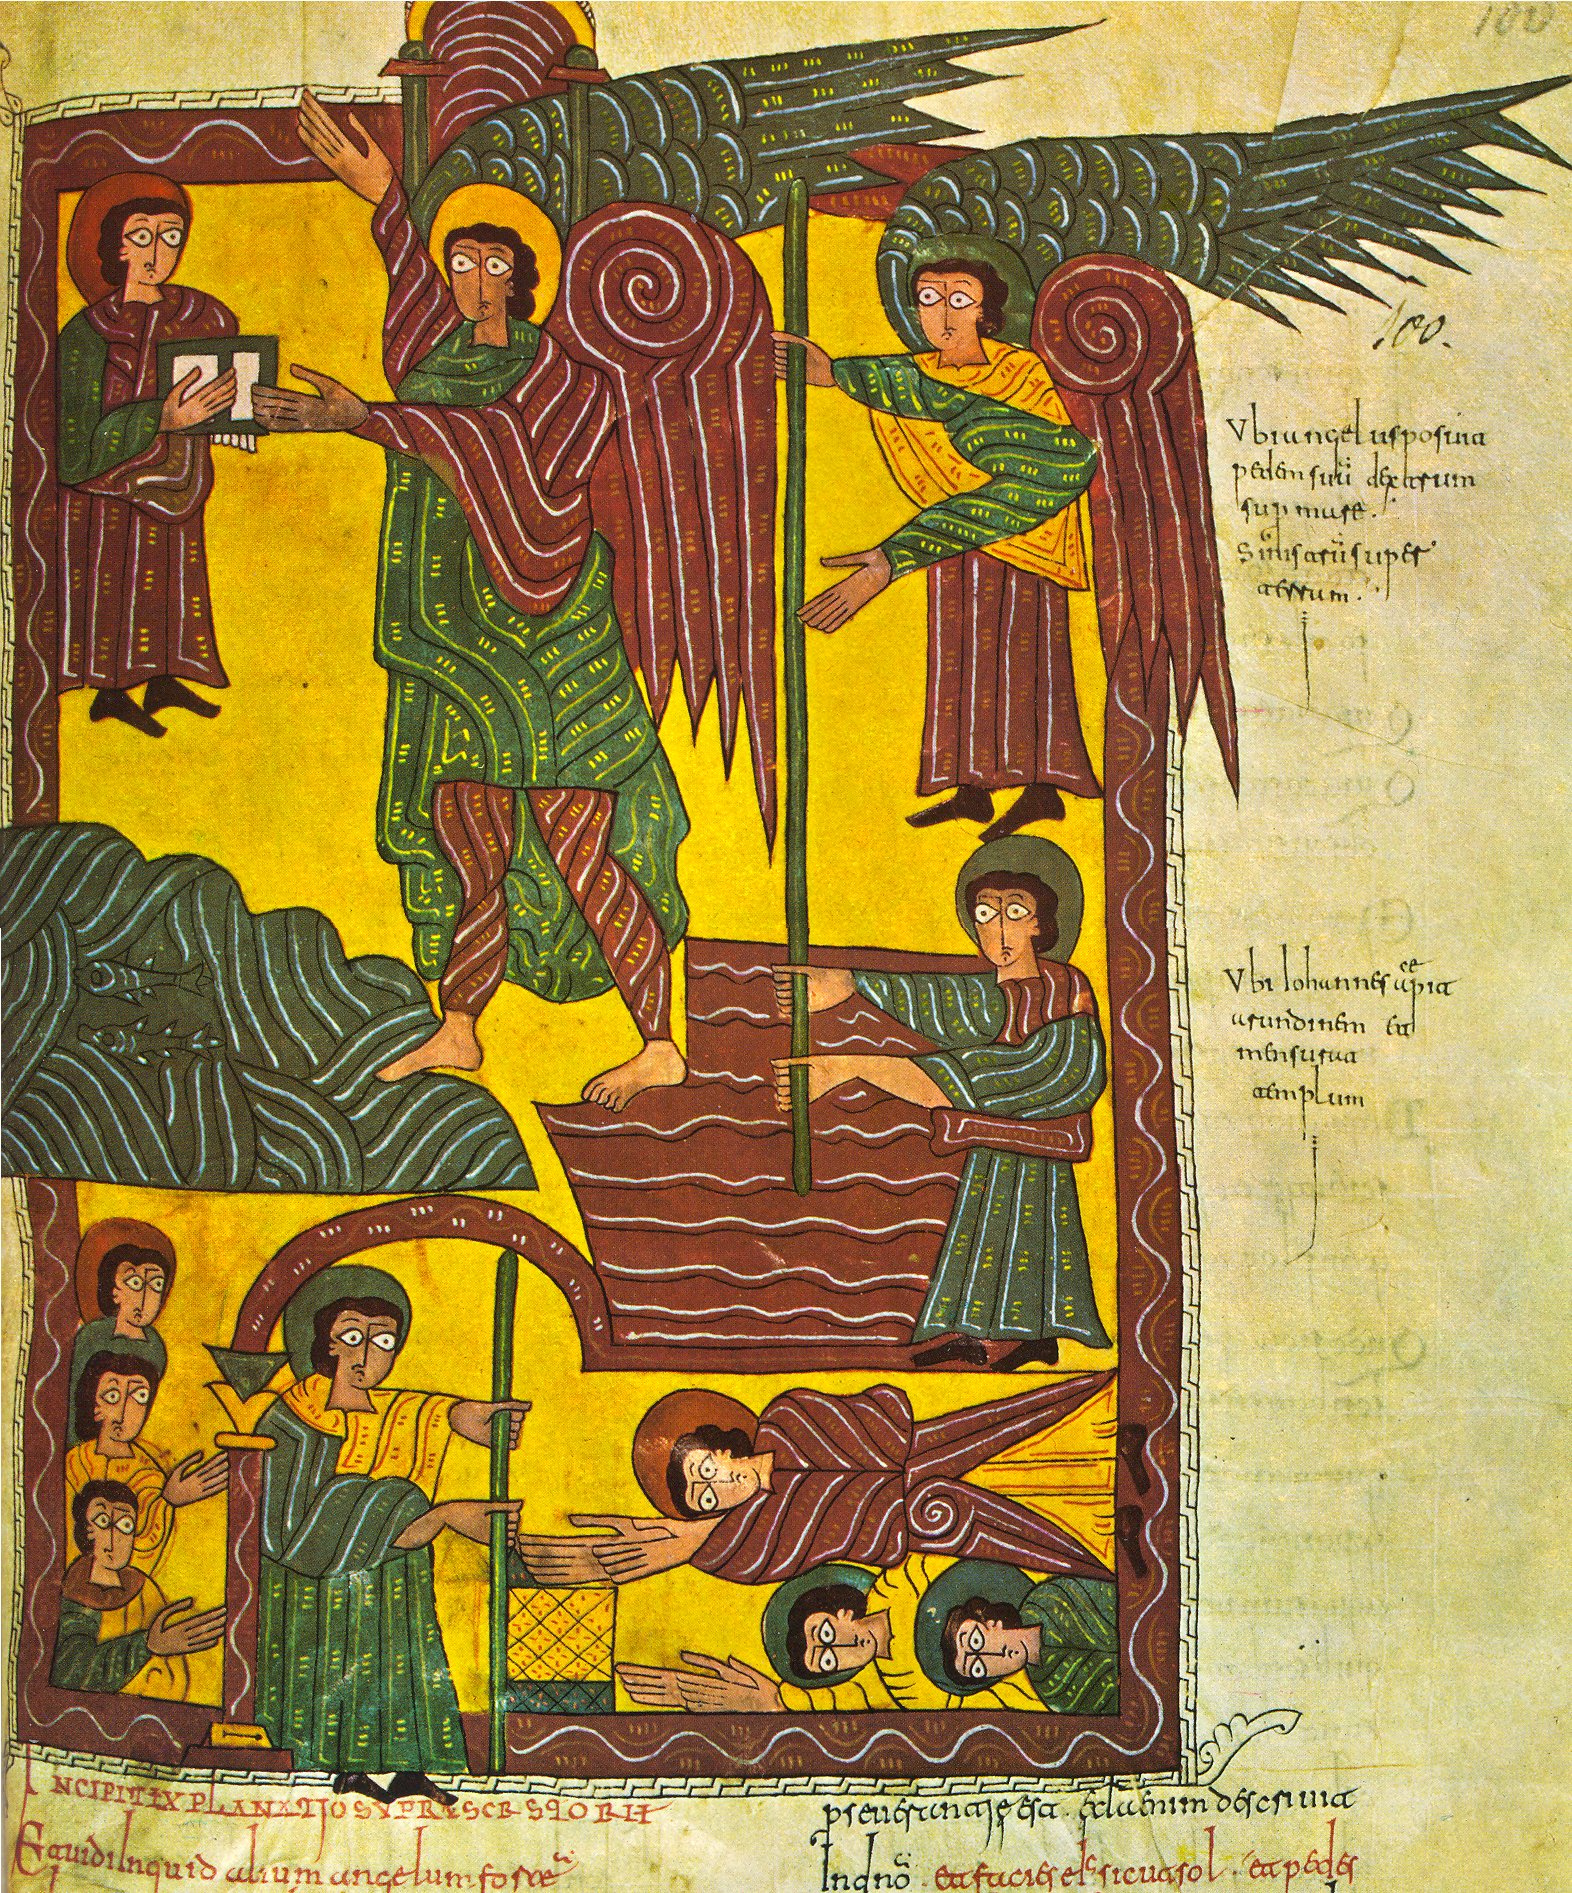
\includegraphics[width=0.95\textwidth]{images/illustrations/facundusmeasuringtemple}
\end{center}